% Generated by system/tools/paper_figures.py from experiments/e3-*/chain.csv; do not edit.
\providecommand{\replaytinggi}{2.5cm}
\definecolor{usulan}{HTML}{2A78D6}
\definecolor{terpicu}{HTML}{EB6834}
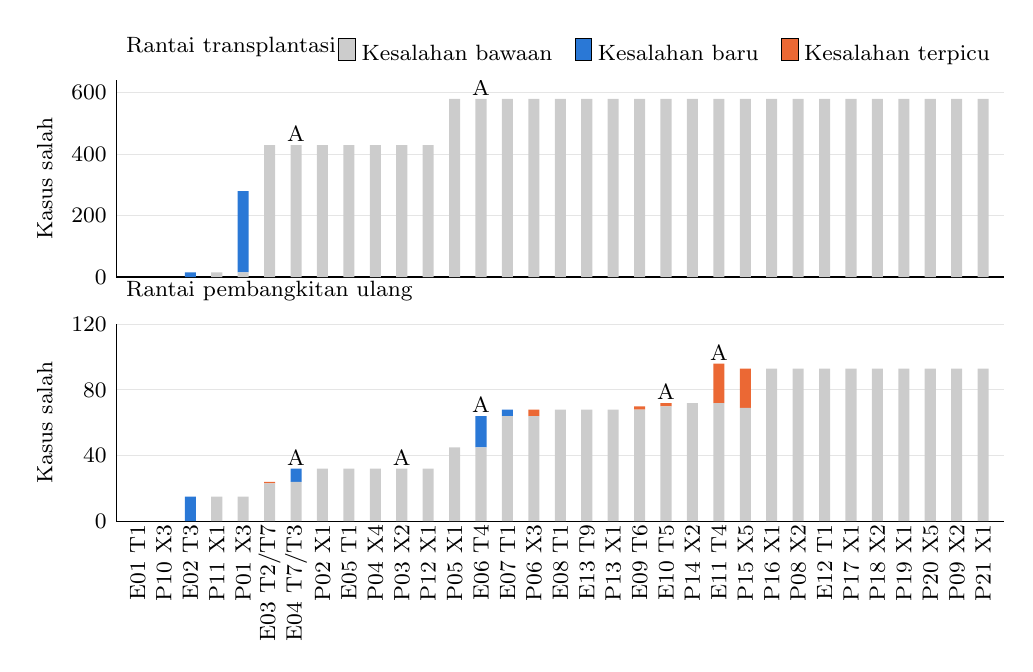
\begin{tikzpicture}
\begin{axis}[name=atas,
  ybar stacked, bar width=4pt, scale only axis, width=0.93\textwidth, height=\replaytinggi,
  xmin=0.2, xmax=33.8, ymin=0, ymax=640, ytick={0,200,400,600},
  xtick={1,...,33}, xticklabels={},
  xtick style={draw=none},
  ylabel={Kasus salah}, label style={font=\footnotesize}, tick label style={font=\footnotesize},
  ymajorgrids, grid style={gray!20, line width=0.3pt}, axis lines*=left, tick style={draw=none},
  title={Rantai transplantasi}, title style={font=\footnotesize, at={(0,1)}, anchor=south west, yshift=-1pt},
  legend style={font=\footnotesize, draw=none, fill=none, at={(1,1.02)}, anchor=south east, legend columns=3, /tikz/every even column/.append style={column sep=6pt}}, reverse legend=false,
]
\addplot[fill=gray!40, draw=none] coordinates {(1,0) (2,0) (3,0) (4,15) (5,15) (6,429) (7,429) (8,429) (9,429) (10,429) (11,429) (12,429) (13,579) (14,579) (15,579) (16,579) (17,579) (18,579) (19,579) (20,579) (21,579) (22,579) (23,579) (24,579) (25,579) (26,579) (27,579) (28,579) (29,579) (30,579) (31,579) (32,579) (33,579)};
\addlegendentry{Kesalahan bawaan}
\addplot[fill=usulan, draw=none] coordinates {(1,0) (2,0) (3,15) (4,0) (5,264) (6,0) (7,0) (8,0) (9,0) (10,0) (11,0) (12,0) (13,0) (14,0) (15,0) (16,0) (17,0) (18,0) (19,0) (20,0) (21,0) (22,0) (23,0) (24,0) (25,0) (26,0) (27,0) (28,0) (29,0) (30,0) (31,0) (32,0) (33,0)};
\addlegendentry{Kesalahan baru}
\addplot[fill=terpicu, draw=none] coordinates {(1,0) (2,0) (3,0) (4,0) (5,0) (6,0) (7,0) (8,0) (9,0) (10,0) (11,0) (12,0) (13,0) (14,0) (15,0) (16,0) (17,0) (18,0) (19,0) (20,0) (21,0) (22,0) (23,0) (24,0) (25,0) (26,0) (27,0) (28,0) (29,0) (30,0) (31,0) (32,0) (33,0)};
\addlegendentry{Kesalahan terpicu}
\node[font=\footnotesize, anchor=south, inner sep=1pt] at (axis cs:7,429) {A};
\node[font=\footnotesize, anchor=south, inner sep=1pt] at (axis cs:14,579) {A};
\end{axis}
\begin{axis}[name=bawah, at={(atas.south west)}, anchor=north west, yshift=-6mm,
  ybar stacked, bar width=4pt, scale only axis, width=0.93\textwidth, height=\replaytinggi,
  xmin=0.2, xmax=33.8, ymin=0, ymax=120, ytick={0,40,80,120},
  xtick={1,...,33}, xticklabels={E01 T1,P10 X3,E02 T3,P11 X1,P01 X3,E03 T2/T7,E04 T7/T3,P02 X1,E05 T1,P04 X4,P03 X2,P12 X1,P05 X1,E06 T4,E07 T1,P06 X3,E08 T1,E13 T9,P13 X1,E09 T6,E10 T5,P14 X2,E11 T4,P15 X5,P16 X1,P08 X2,E12 T1,P17 X1,P18 X2,P19 X1,P20 X5,P09 X2,P21 X1},
  xticklabel style={rotate=90, anchor=east, font=\footnotesize, inner sep=1pt},
  ylabel={Kasus salah}, label style={font=\footnotesize}, tick label style={font=\footnotesize},
  ymajorgrids, grid style={gray!20, line width=0.3pt}, axis lines*=left, tick style={draw=none},
  title={Rantai pembangkitan ulang}, title style={font=\footnotesize, at={(0,1)}, anchor=south west, yshift=-1pt},
  legend style={draw=none},
]
\addplot[fill=gray!40, draw=none] coordinates {(1,0) (2,0) (3,0) (4,15) (5,15) (6,23) (7,24) (8,32) (9,32) (10,32) (11,32) (12,32) (13,45) (14,45) (15,64) (16,64) (17,68) (18,68) (19,68) (20,68) (21,70) (22,72) (23,72) (24,69) (25,93) (26,93) (27,93) (28,93) (29,93) (30,93) (31,93) (32,93) (33,93)};
\addplot[fill=usulan, draw=none] coordinates {(1,0) (2,0) (3,15) (4,0) (5,0) (6,0) (7,8) (8,0) (9,0) (10,0) (11,0) (12,0) (13,0) (14,19) (15,4) (16,0) (17,0) (18,0) (19,0) (20,0) (21,0) (22,0) (23,0) (24,0) (25,0) (26,0) (27,0) (28,0) (29,0) (30,0) (31,0) (32,0) (33,0)};
\addplot[fill=terpicu, draw=none] coordinates {(1,0) (2,0) (3,0) (4,0) (5,0) (6,1) (7,0) (8,0) (9,0) (10,0) (11,0) (12,0) (13,0) (14,0) (15,0) (16,4) (17,0) (18,0) (19,0) (20,2) (21,2) (22,0) (23,24) (24,24) (25,0) (26,0) (27,0) (28,0) (29,0) (30,0) (31,0) (32,0) (33,0)};
\node[font=\footnotesize, anchor=south, inner sep=1pt] at (axis cs:7,32) {A};
\node[font=\footnotesize, anchor=south, inner sep=1pt] at (axis cs:11,32) {A};
\node[font=\footnotesize, anchor=south, inner sep=1pt] at (axis cs:14,64) {A};
\node[font=\footnotesize, anchor=south, inner sep=1pt] at (axis cs:21,72) {A};
\node[font=\footnotesize, anchor=south, inner sep=1pt] at (axis cs:23,96) {A};
\end{axis}
\end{tikzpicture}
